\documentclass{beamer}
\usepackage[utf8]{inputenc}
\usepackage{bm}
\usepackage{tikz}
\usepackage{amsmath}
\usetikzlibrary{arrows}

\usetheme{Madrid}
\usecolortheme{default}


%------------------------------------------------------------
%This block of code defines the information to appear in the
%Title page
\title[An Interesting Lebesgue Intergrable Function] %optional
{An Interesting Lebesgue Intergrable Function}

% \subtitle{A short story}

\author[H.~Han]
{H.~Han}

% \institute[VFU] % (optional)
% {
%   \inst{1}%
%   Faculty of Physics\\
%   Very Famous University
%   \and
%   \inst{2}%
%   Faculty of Chemistry\\
%   Very Famous University
% }

% \date[VLC 2021] % (optional)
% {Very Large Conference, April 2021}


%End of title page configuration block
%------------------------------------------------------------



%------------------------------------------------------------
%The next block of commands puts the table of contents at the 
%beginning of each section and highlights the current section:

% \AtBeginSection[]
% {
%   \begin{frame}
%     \frametitle{Table of Contents}
%     \tableofcontents[currentsection]
%   \end{frame}
% }
%------------------------------------------------------------


\begin{document}

%The next statement creates the title page.
\frame{\titlepage}


%---------------------------------------------------------
%This block of code is for the table of contents after
%the title page
% \begin{frame}
% \frametitle{Table of Contents}
% \tableofcontents
% \end{frame}
%---------------------------------------------------------


\section{First section}

%---------------------------------------------------------
%Changing visivility of the text
% \begin{frame}
% \frametitle{Sample frame title}
% This is a text in second frame. For the sake of showing an example.
%
% \begin{itemize}
%     \item<1-> Text visible on slide 1
%     \item<2-> Text visible on slide 2
%     \item<3> Text visible on slides 3
%     \item<4-> Text visible on slide 4
% \end{itemize}
% \end{frame}

%---------------------------------------------------------


%---------------------------------------------------------
%Example of the \pause command
% \begin{frame}
% In this slide \pause
%
% the text will be partially visible \pause
%
% And finally everything will be there
% \end{frame}
%---------------------------------------------------------

% \section{Second section}

%---------------------------------------------------------
\begin{frame}
\frametitle{Lebesgue Intergral is a Generalization of Riemann Integral}

\begin{block}{All Reimain Integrable Functions are Lebesgue Integrable}
\end{block}

\begin{alertblock}{\textbf{Not} All Lebesgue Integrable Functions are Reimann Integrable}
	Classic Example: Dirichlet Functions
	\[
		\mathcal{D}(x) =
		\begin{cases}
			1 & x \in \mathbb{Q} \\
			0 & x \notin \mathbb{Q}
		\end{cases}
	\]
	We have:
	$$(L) \int \mathcal{D} = 0$$
	As Lebesgue integral over countable set is 0. 
\end{alertblock}


% \begin{alertblock}{Important theorem}
% Sample text in red box
% \end{alertblock}
%
% \begin{examples}
% Sample text in green box. The title of the block is ``Examples".
% \end{examples}
\end{frame}

\begin{frame}
\frametitle{An Interesting Example}

\begin{block}{Example}
	Consider function
	\[ 
		f(x) = \frac{1}{x^{1/2}}
	\]
	This function is clearly not Reimainn Integrable over $I = (0, 1]$.

	However, I claim that:
	\[ 
		(L) \int_{0}^{1} f(x) = 2
	\]

	\begin{figure}
		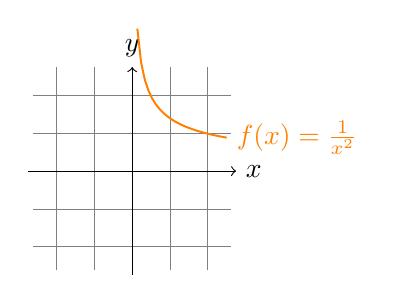
\begin{tikzpicture}[scale = 0.6,domain=-0.2:2]
			\draw[step=0.8, very thin,color=gray] (-2.1,-2.1) grid (2.1,2.2);
			\draw[->] (-2.2,0) -- (2.2,0) node[right] {$x$};
			\draw[->] (0,-2.2) -- (0,2.2) node[above] {$y$};
			\draw[color=orange, line width = 0.25mm, domain=0.11:2] plot (\x,{1/((\x)^(1/2))}) node[right] {$f(x) = \frac{1}{x^{2}}$};
		\end{tikzpicture}
	\end{figure}
\end{block}

\end{frame}

\begin{frame}
\frametitle{Justification : $ (L) \int_{0}^{1} f(x) dx = 2 $}

\begin{block}{Example}
	$f(x)$ has inverse function $g(x) = x^2$.

	Thus: 
	\[ 
		(L) \int_{0}^{1} \frac{1}{x^{1/2}} = 1 + (R) \int_{1}^{\infty} \frac{1}{x^2} = 2
	\]
	\begin{figure}
		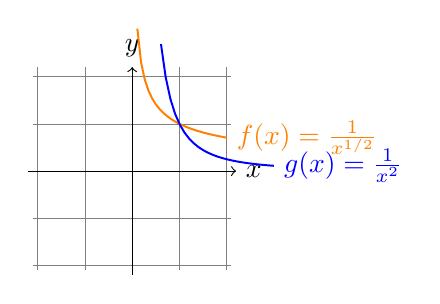
\begin{tikzpicture}[scale = 0.6,domain=-0.2:2]
			\draw[step=1, very thin,color=gray] (-2.1,-2.1) grid (2.1,2.2);
			\draw[->] (-2.2,0) -- (2.2,0) node[right] {$x$};
			\draw[->] (0,-2.2) -- (0,2.2) node[above] {$y$};
			\draw[color=orange, line width = 0.25mm, domain=0.11:2] plot (\x,{1/((\x)^(1/2))}) node[right] {$f(x) = \frac{1}{x^{1/2}}$};
			\draw[color=blue, line width = 0.25mm, domain=0.61:3] plot (\x,{1/((\x)^(2))}) node[right] {$g(x) = \frac{1}{x^{2}}$};
		\end{tikzpicture}
	\end{figure}
\end{block}

\end{frame}


%---------------------------------------------------------
%Two columns
% \begin{frame}
% \frametitle{Two-column slide}
%
% \begin{columns}
%
% \column{0.5\textwidth}
% This is a text in first column.
% $$E=mc^2$$
% \begin{itemize}
% \item First item
% \item Second item
% \end{itemize}
%
% \column{0.5\textwidth}
% This text will be in the second column
% and on a second tought this is a nice looking
% layout in some cases.
% \end{columns}
% \end{frame}
%---------------------------------------------------------


\end{document}
